\documentclass[12pt]{article}
\usepackage{url,graphicx,tabularx,array}
\usepackage[margin=1in]{geometry}
\setlength{\parskip}{1ex} %--skip lines between paragraphs
\setlength{\parindent}{0pt} %--don't indent paragraphs

\usepackage{algorithmic}
\usepackage{algorithm}
\usepackage{ amssymb }
\usepackage{ latexsym }
\usepackage{ amsmath }
\usepackage{ amsthm }
%-- Commands for header
\renewcommand{\title}[1]{\textbf{#1}\\}
\renewcommand{\line}{\begin{tabularx}{\textwidth}{X>{\raggedleft}X}\hline\\\end{tabularx}\\[-0.5cm]}
\newcommand{\leftright}[2]{\begin{tabularx}{\textwidth}{X>{\raggedleft}X}#1%
& #2\\\end{tabularx}\\[-0.5cm]}

\newtheorem{defn}{Definition}[section]
\newtheorem{conjecture}{conjecture}[section]
\newtheorem{lemma}{Lemma}[section]
\newtheorem{corollary}{Corollary}[section]
\newtheorem{question}{Question}[section]
\newtheorem{proposition}{Proposition}[section]


%\linespread{2} %-- Uncomment for Double Space
\begin{document}

\title{Homework 6: CMPS 242}
\line
\leftright{\today}{Bryan Matsuo (bmatsuo@soe.ucsc.edu) \& John St. John (jstjohn@soe.ucsc.edu)} %-- left and right positions in the header
\begin{enumerate}
\item \textbf{AdaBoost:}

Following is the work for an AdaBoost run given the data in Table~\ref{tab:adaData}. In the following equations, let $Q_t(i) = D_t(i) \exp(-\alpha_t y_i h_t(x_i))$. At the end of the following iterations is the final Master Hypothesis.

\textit{ Iteration 1:}
\begin{eqnarray*}
t=1, D_1(i) = \frac{1}{4} \\
\Pr_{\text{error} \sim D_1}\left(f_1\right) = \Pr_{\text{error} \sim D_1}\left(f_2\right)= \Pr_{\text{error} \sim D_1}\left(f_3\right) = \frac{1}{4} \\
h_1 = f_1, e_1 = \frac{1}{4}, \alpha_1 = \frac{1}{2} \ln 3 \\
Q_1(1) = \frac{1}{4} \exp \left( -\frac{1}{2}  \ln 3 \right) = \frac{1}{4\sqrt{3}} \\
Q_1(2) = \frac{1}{4} \exp \left( -\frac{1}{2}  \ln 3 \right) = \frac{1}{4\sqrt{3}} \\
Q_1(3) = \frac{1}{4} \exp \left( \frac{1}{2}  \ln 3 \right) =\frac{\sqrt{3}}{4}\\
Q_1(4) = \frac{1}{4} \exp \left( -\frac{1}{2}  \ln 3 \right)= \frac{1}{4\sqrt{3}}  \\
\text{norm}_1 = \frac{3}{4\sqrt{3}} + \frac{\sqrt{3}}{4} = \frac{6}{4\sqrt{3}} \\
D_2(1,2,4) = \frac{1}{4\sqrt{3}} \frac{4\sqrt{3}}{6} = \frac{1}{6}\\
D_2(3) = \frac{\sqrt{3}}{4}\frac{4\sqrt{3}}{6} = \frac{1}{2}
\end{eqnarray*}

\textit{ Iteration 2:}
\begin{eqnarray*}
t=2\\
\Pr_{\text{error} \sim D_2}\left(f_1\right) = \frac{1}{2} \\
\Pr_{\text{error} \sim D_2}\left(f_2\right)= \Pr_{\text{error} \sim D_2}\left(f_3\right) = \frac{1}{6} \\
h_2 = f_2, e_2 = \frac{1}{6}, \alpha_2 = \frac{1}{2} \ln 5 \\ 
Q_2(1) = \frac{1}{6} \exp \left( -\frac{1}{2}  \ln 3 \right) = \frac{1}{6\sqrt{5}} \\
Q_2(2) = \frac{1}{6} \exp \left( \frac{1}{2}  \ln 3 \right) = \frac{\sqrt{5}}{6} \\
Q_2(3) = \frac{1}{2} \exp \left( -\frac{1}{2}  \ln 3 \right) =\frac{1}{2\sqrt{5}}\\
Q_2(4) = \frac{1}{6} \exp \left( -\frac{1}{2}  \ln 3 \right)= \frac{1}{6\sqrt{5}}  \\
\text{norm}_2 = \frac{2}{6\sqrt{5}} + \frac{1}{2\sqrt{5}}\left(\frac{3}{3}\right) + \frac{\sqrt{5}}{6}\left(\frac{\sqrt{5}}{\sqrt{5}} \right)= \frac{10}{6\sqrt{5}} \\
D_3(1,4) =  \frac{1}{6\sqrt{5}} \left(\frac{6\sqrt{5}}{10}\right) = \frac{1}{10}\\
D_3(2) = \frac{\sqrt{5}}{6} \left(\frac{6\sqrt{5}}{10}\right) = \frac{1}{2}\\
D_3(3) = \frac{1}{2\sqrt{5}} \left(\frac{6\sqrt{5}}{10}\right) = \frac{3}{10}
\end{eqnarray*}

\textit{ Iteration 3 (final):}
\begin{eqnarray*}
t=3\\
\Pr_{\text{error} \sim D_3}\left(f_1\right) = \frac{3}{10} \\
\Pr_{\text{error} \sim D_3}\left(f_2\right)= \frac{1}{2} \\
\Pr_{\text{error} \sim D_3}\left(f_3\right) = \frac{1}{10} \\
h_3 = f_3, e_3 = \frac{1}{10}, \alpha_3 = \frac{1}{2} \ln 9
\end{eqnarray*}

\textit{Master Hypothesis:}
\begin{eqnarray*}
H(X) = \text{sign}\left[  \frac{1}{2}\left(\ln(3) f_1(x) +  \ln(5) f_2(x) + \ln(9) f_3(x)   \right)\right] \\
 = \text{sign} \left(\ln(3) f_1(x) +  \ln(5) f_2(x) + \ln(9) f_3(x) \right)
\end{eqnarray*}



\begin{table}[htdp]
\caption{AdaBoost training data.}
\begin{center}
\begin{tabular}{|l|c||c|c|c|}
\hline
instance & label & $f_1$ & $f_2$ & $f_3$ \\
\hline
$x_1$ &  -1 &  -1 &  -1 & +1 \\
$x_2$ & +1 & +1 &  -1 & +1 \\
$x_3$ & +1 &  -1 & +1 & +1 \\
$x_4$ & +1 & +1 & +1 & +1 \\
\hline
\end{tabular}
\end{center}
\label{tab:adaData}
\end{table}%



\item \textbf{T base learners:}

Let $C_t \in \{0,1\}$ be  the event that learner $t$ predicts correctly. All $C_t$ are independent, and the $\Pr(C_t=1) = p$. The majority prediction of the learners is correct is $\sum_{t=1}^TC_t > \left\lfloor \frac{T}{2} \right\rfloor $. Because $C_t$ is a Bernoulli random variable, their sum is a binomial with parameters $T$ and $p$. The probability of a correct majority of votes becomes $1-F\left(\left\lfloor\frac{T}{2}\right\rfloor\right)$ where $F(x)$ is the CDF of a binomial with parameters $T$ and $p$. 
\begin{equation}
\Pr(\text{Correct Majority}) = 1- \sum_{k=0}^{\left\lfloor T/2 \right\rfloor} {T \choose k}p^k(1-p)^{T-k}
\end{equation}

\begin{figure}[htbp]
\begin{center}
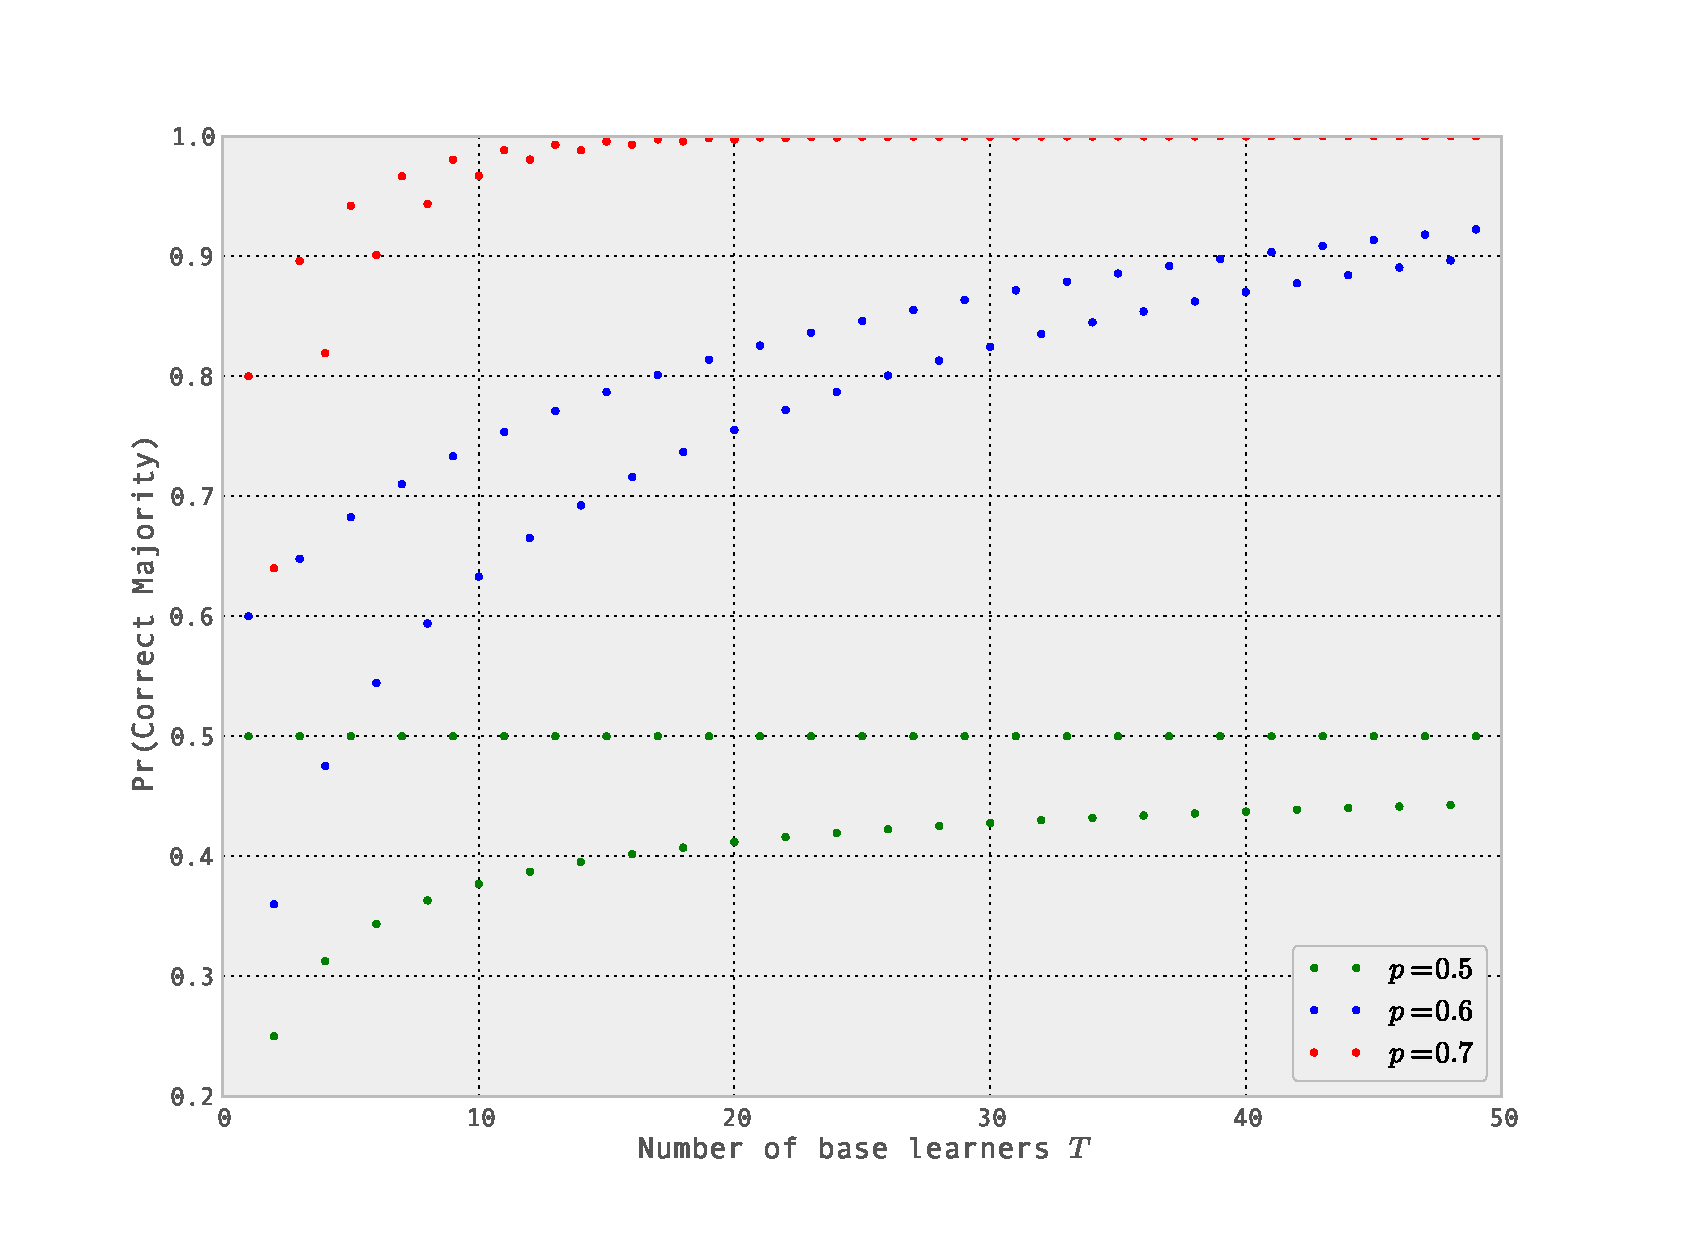
\includegraphics[scale=0.55]{prob2.eps}
\caption{Plot of probability of voting, given different probabilities of votes, and numbers of voters.}
\label{fig:prob2}
\end{center}
\end{figure}


\item \textbf{EM Clustering:}

Since each of the gaussians share all of the points with the same weight, they start off exactly the same. Since the update does not incorporate a randomizer, and each of the gaussians are updated in one step, they will all be updated deterministically in the same way. This means they will always be the same gaussians.

\end{enumerate}
\end{document}
